\documentclass[border=10pt]{standalone}
\usepackage{tikz}
\usetikzlibrary{arrows.meta, positioning}
\definecolor{myblue}{RGB}{0, 70, 165}
\definecolor{myteal}{RGB}{0, 120, 120}
\definecolor{myorange}{RGB}{237, 124, 0}
\definecolor{myred}{RGB}{190, 0, 40}
\tikzset{
  >={Stealth[width=2.2mm,length=2.2mm]},
  base/.style = {rectangle, rounded corners, draw=myblue, very thick,
    minimum width=4cm, minimum height=1cm, text centered, font=\sffamily\bfseries, text=myblue},
  startstop/.style = {base, fill=myred!18, draw=myred, text=myred},
  logicblock/.style = {base, fill=myteal!20, draw=myteal, font=\sffamily\itshape, text=myteal},
  process/.style = {base, minimum width=2.8cm, fill=myorange!15, draw=myorange, font=\ttfamily, text=myorange},
}

\begin{document}
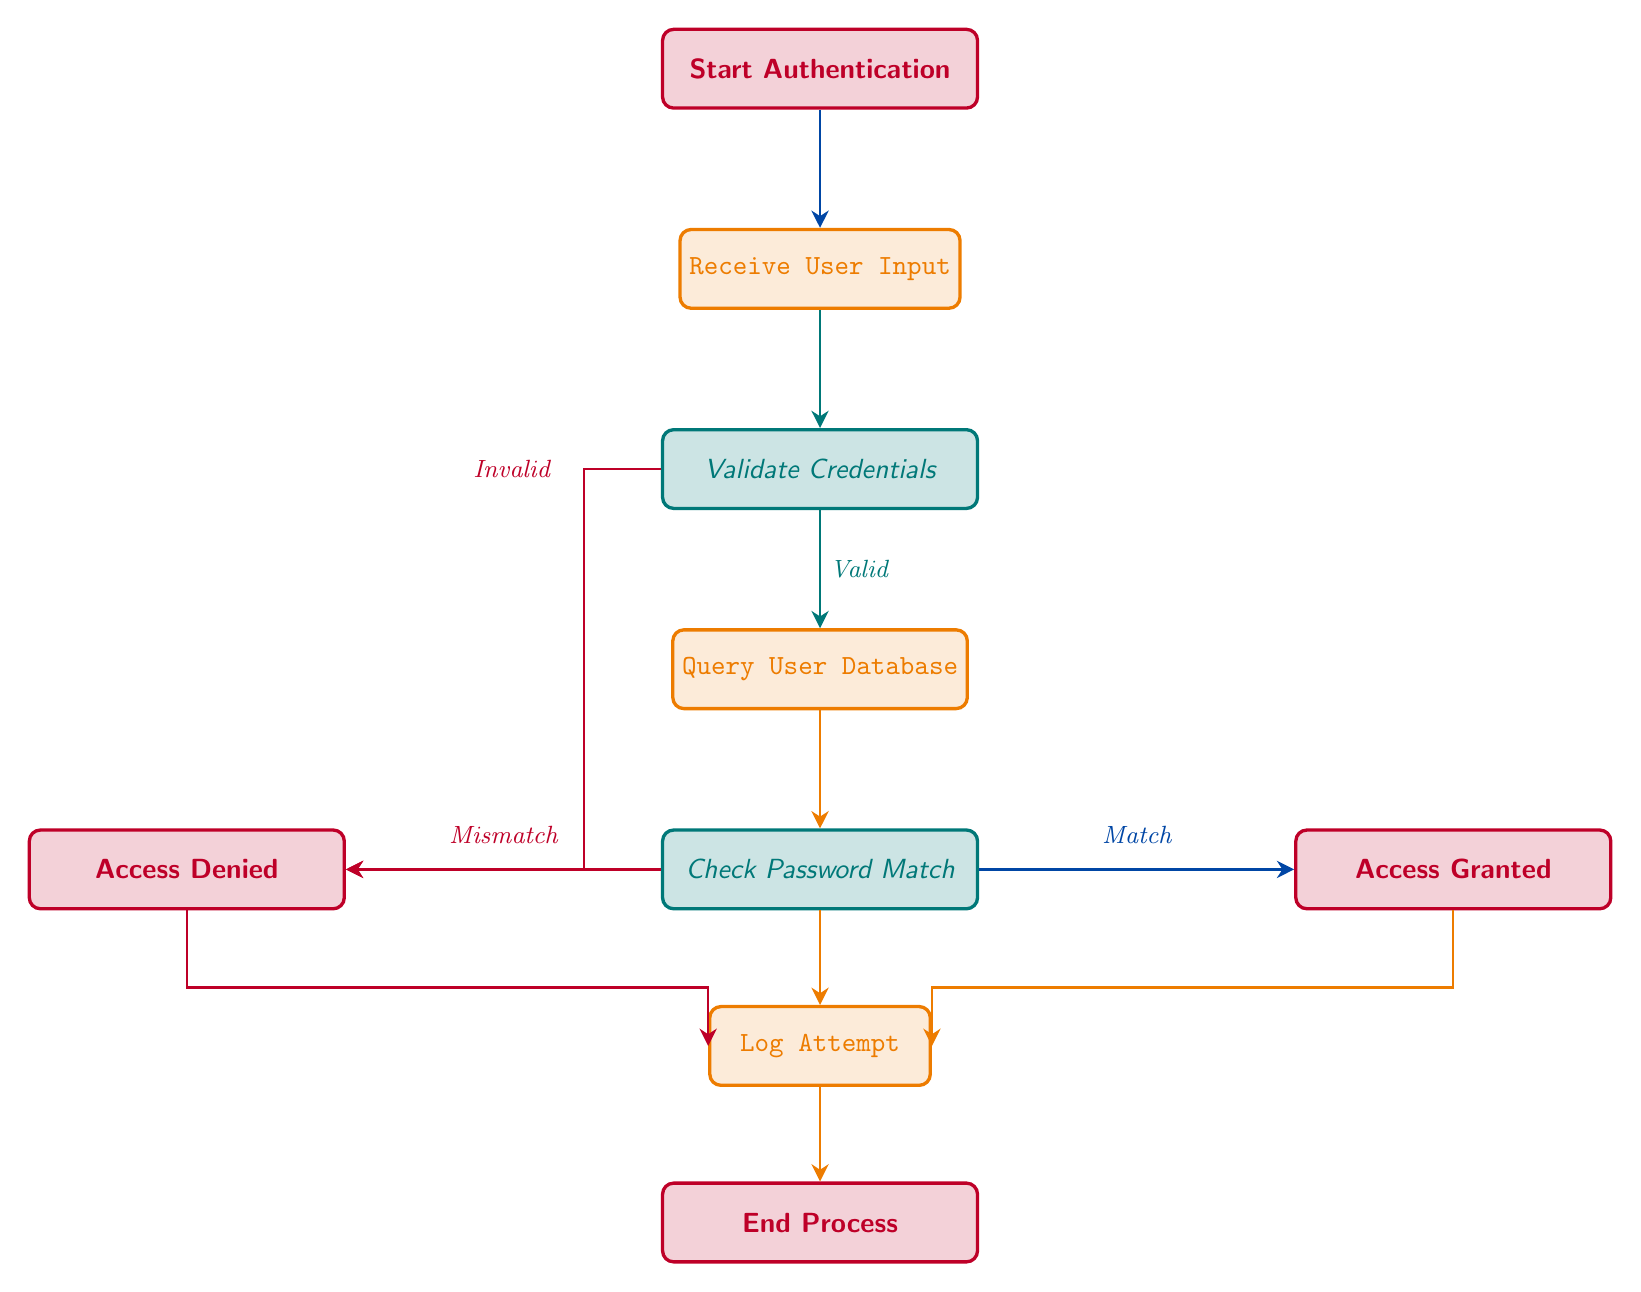
\begin{tikzpicture}[node distance=1.5cm, align=center]
  % Nodes for a flowchart of a basic login authentication process
  \node (start)             [startstop]              {Start Authentication};
  \node (getInput)          [process, below=of start] {Receive User Input};
  \node (validateInput)     [logicblock, below=of getInput] {Validate Credentials};
  \node (checkDB)           [process, below=of validateInput] {Query User Database};
  \node (verify)            [logicblock, below=of checkDB] {Check Password Match};
  \node (accessGranted)     [startstop, right=4cm of verify] {Access Granted};
  \node (accessDenied)      [startstop, left=4cm of verify] {Access Denied};
  \node (logAttempt)        [process, below=1.2cm of verify] {Log Attempt};
  \node (end)               [startstop, below=1.2cm of logAttempt] {End Process};

  % Arrows
  \draw[->, thick, myblue] (start) -- (getInput);
  \draw[->, thick, myteal] (getInput) -- (validateInput);
  \draw[->, thick, myteal] (validateInput) -- node[right, text=myteal, font=\small\itshape] {Valid} (checkDB);
  \draw[->, thick, myred] (validateInput) -- ++(-3,0) node[left, text=myred, font=\small\itshape, xshift=-0.3cm] {Invalid} |- (accessDenied);
  \draw[->, thick, myorange] (checkDB) -- (verify);
  \draw[->, thick, myblue] (verify) -- node[above, text=myblue, font=\small\itshape, yshift=0.2cm] {Match} (accessGranted);
  \draw[->, thick, myred] (verify) -- node[above, text=myred, font=\small\itshape, yshift=0.2cm] {Mismatch} (accessDenied);
  \draw[->, thick, myorange] (verify) -- (logAttempt);
  \draw[->, thick, myorange] (logAttempt) -- (end);
  \draw[->, thick, myorange] (accessGranted) |- ++(0,-1.5) -| (logAttempt.east);
  \draw[->, thick, myred] (accessDenied) |- ++(0,-1.5) -| (logAttempt.west);
\end{tikzpicture}
\end{document}